We present world averages of a selection of \mtau lepton quantities lepton
that most benefit from the adoption of the HFAG
methodology~\cite{Asner:2010qj}.
All published statistical correlations are used, and a
selection of measurements, particularly the most precise and the most
recent, were studied to take into account the significant systematic
dependencies from external parameters and common systematic sources.

Particular care has been used to engineer a global fit of the \mtau
branching fractions (Section~\ref{sec:tau:br-fit}) to obtain consistent
and statistically complete information for further elaboration in order to
compute lepton universality tests (Section~\ref{sec:tau:leptonuniv}) and
the CKM matrix element $|V_{us}|$ (Section~\ref{sec:tau:vus}).

Finally, we report in Section~\ref{sec:tau:lfv} the most up-to-date limits
on the lepton-flavour-violating tau branching fractions and, starting with
this report, we also provide combined upper limits.

%% ///////////////////////////////////////////////////////////////////////////
\tausection{Branching fractions fit}
\cutname{br-fit.html}
\label{sec:tau:br-fit}

The measurements listed in Table~\ref{tab:tau:br-fit} have been used in a
minimum \chisq fit subject to the constraints that are listed
either in the same table (where some fitted quantities and experimental
measurements are expressed as ratios of fit quantities) or in
Section~\ref{sec:tau:constraints}. The fitted quantities and the measurements
are labelled using the PDG~\cite{PDG_2010} $\Gamma_{n}$ notation, where $n$ is
an integer number, which matches the PDG notation for $n<800$. We use
$n\ge 800$ to denote some additional branching fractions, as documented in the
former HFAG report~\cite{Asner:2010qj}. The PDG $\Gamma_{n}$ notation does
not maintain the same numbers across editions. We continue using the PDG
2010 numbers with the aim to eventually switch to a different stable notation,
probably based on PDG identifiers~\cite{pdg-identifiers-2014}.

The fitted branching fractions consist on \HfagTauBaseQuantNum ``base nodes'' and \HfagTauConstrNum derived
branching fractions, described either as sum of base nodes (see
Section~\ref{sec:tau:constraints}) or as ratios of branching fractions (see
Table~\ref{tab:tau:br-fit}). Furthermore, we define (see
Section~\ref{sec:tau:constraints}) $\Gamma_{\text{All}}$ as the sum of all
the base modes, which correspond to all non-overlapping tau decay modes,
$\Gamma_{998} = 1 -\Gamma_{\text{All}}$ and $\Gamma_{110} =
\BRF{\tau^-}{X_s^- \nu_\tau}$, which is the total branching fraction of the
tau to modes with the strangeness quantum number equal to one.

The fitted \hfagtau averages are reported in
Table~\ref{tab:tau:br-fit}. The fit has $\chi^2/\text{d.o.f.} = \HfagTauChisq/\HfagDof$,
corresponding to a confidence level $\text{CL} = \HfagTauChisqProb$. We use a total of
\HfagTauMeasNum measurements to fit the above mentioned \HfagTauQuantNum quantities.
The fit is statistically consistent with the unitarity constraint, but the
unitarity constraint is not applied.

In several cases, when it is statistically equivalent within the \hfagtau
fitting procedure, for historical reasons the statistical and systematic
errors are added in quadrature and are reported in the above table in the
location of the statistical error, reporting zero as systematic error. A
scale factor of 5.44 (as in the two previous reports
report~\cite{Asner:2010qj,Amhis:2012bh}) has been applied to the published
uncertainties of the two severely inconsistent measurements of
\(\Gamma_{96} = \tau \to KKK\nu\) by \babar and Belle, following the same
procedure as the PDG.

\tausubsection{Changes with respect to the previous report}

The following additions and changes gave been done with respect to the 2012
report~\cite{Amhis:2012bh}.

Published results from two \babar papers and one Belle paper have been
added. The following results have been used from the \htuse{LEES 2012X.collab} high
multiplicity decay \mtau braching fractions paper~\htuse{LEES 2012X.cite}:
{\setlength{\LTleft}{\parindent}%
\begin{longtable}{@{}ll@{}}
\htuse{LEES 2012X.meas}.
\end{longtable}}
\noindent The former $\tau^- \to \htuse{Gamma136.td}$
result~\cite{Aubert:2008nj} is superseded by the above one.  The following
results have been used from the \htuse{LEES 2012Y.collab} paper on the
\mtau branching fractions with two
$K_S$~\htuse{LEES 2012Y.cite}:
{\setlength{\LTleft}{\parindent}%
\begin{longtable}{@{}ll@{}}
\htuse{LEES 2012Y.meas},
\end{longtable}}
\noindent Finally, the following results have been used from the
\htuse{Ryu:2014vpc.collab} paper on the $K_S$ final
states~\htuse{Ryu:2014vpc.cite}:
{\setlength{\LTleft}{\parindent}%
\begin{longtable}{@{}ll@{}}
\htuse{Ryu:2014vpc.meas},
\end{longtable}}
\noindent these results supersede the preliminary ones~\cite{SooRyu:2011aa}
and the former published result on $\tau^- \to \htuse{Gamma35.td}$~\cite{Epifanov:2007rf}.
In order to profit from the measurements of branching fractions with two
$K_S$ in the final state, we drop the inclusive ALEPH measurement on
$\tau^- \to \htuse{Gamma49.td}$~\cite{Barate:1999hj} and we add the esclusive ALEPH
measurement on $\tau^- \to \htuse{Gamma51.td}$~\cite{Barate:1999hj}.

In order to best integrate the above new results in the global fit, the following
constraints have been added:
{\setlength{\LTleft}{\parindent}%
\begin{tabularx}{\linewidth-\parindent}{@{}lX@{}}
  \htuse{Gamma13.c.constr.eq} \\
  \htuse{Gamma33.c.constr.eq} \\
  \htuse{Gamma49.c.constr.eq} \\
  \htuse{Gamma78.c.constr.eq} \\
  \htuse{Gamma103.c.constr.eq} \\
  \htuse{Gamma104.c.constr.eq} \\
  \htuse{Gamma806.c.constr.eq} \\
  \htuse{Gamma810.c.constr.eq} \\
  \htuse{Gamma820.c.constr.eq} \\
  \htuse{Gamma830.c.constr.eq} \\
  \htuse{Gamma910.c.constr.eq} \\
  \htuse{Gamma930.c.constr.eq} \\
  \htuse{Gamma944.c.constr.eq} \\
  \htuse{Gamma911.c.constr.eq}~.
\end{tabularx}}
The definition of the total branching fraction and of the inclusive
tranching fraction of the \mtau lepton into a strange final states have
been updated as follows:
{\setlength{\LTleft}{\parindent}%
\begin{tabularx}{\linewidth-\parindent}{@{}lX@{}}
  \htuse{Gamma110.c.constr.eq} \\
  \htuse{GammaAll.c.constr.eq}~.
\end{tabularx}}
\noindent Finally, a wrong constraint used in the two previous reports has been
removed:
{\setlength{\LTleft}{\parindent}%
\begin{tabularx}{\linewidth-\parindent}{@{}lX@{}}
  $\Gamma_{136}$ ={}& $\Gamma_{104}\cdot \Gamma_{\eta \to \pi^+\pi^-\pi^0} +
  \Gamma_{78} \cdot \Gamma_{\eta \to 3\pi^0}$~.
\end{tabularx}}
\noindent The wrong constraint has been affecting in a negligible way the
global fit, except for the involved specific branching ratios.
In particular, the effects on the lepton universality tests and
in the \Vus determination were negligible.

Finally, the constraint parameters (see Section~\ref{sec:tau:constraints})
have been updated to the PDG 2013 results~\cite{PDG_2013}.

%%
%% quantities and measurements
%%
\begin{center}
\begin{envsmall}
\setlength{\LTcapwidth}{0.85\linewidth}
\renewcommand*{\arraystretch}{1.3}%
\ifhevea
\renewcommand{\bar}[1]{\textoverline{#1}}
\else
\makeatletter
%%--- prevent longtable to go over page number
\@lowpenalty=5
\makeatother
\fi
\begin{longtable}{llll}
\caption{HFAG Winter 2012 branching fractions fit results.\label{tab:tau:br-fit}}%
\\
\hline
\multicolumn{1}{l}{\bfseries Tau lepton branching fraction} &
\multicolumn{1}{l}{\bfseries Value} &
\multicolumn{1}{l}{\bfseries Exp.} &
\multicolumn{1}{l}{\bfseries Ref.} \\
\hline
\endfirsthead
\multicolumn{4}{c}{{\bfseries \tablename\ \thetable{} -- continued from previous page}} \\ \hline
\multicolumn{1}{l}{\bfseries Tau lepton branching fraction} &
\multicolumn{1}{l}{\bfseries Value} &
\multicolumn{1}{l}{\bfseries Exp.} &
\multicolumn{1}{l}{\bfseries Ref.} \\
\hline
\endhead
\endfoot
\endlastfoot
\HfagTauBrVal \\
\hline
\end{longtable}
\end{envsmall}
\end{center}

\tausubsection{Correlation between base nodes uncertainties}
\label{sec:tau:fitcorr}

The following tables report the correlation coefficients between base nodes,
in percent.

%%
%% base nodes correlations
%%
\HfagTauBrCorr

\tausubsection{Equality constraints}
\label{sec:tau:constraints}

We use equality constraints that relate a branching fraction to a sum of
branching fractions. As mentioned above, the tau branching fractions are
denoted with $\Gamma_n$ labels. In the constraint relations we use the
values of some non-tau branching fractions, denoted e.g.\ with the
self-describing notation $\Gamma_{K_S \to \pi^0\pi^0}$. We also use
probabilities corresponding to modulus square amplitudes describing quantum
mixtures of states such as $K^0$, $\bar{K}^0$, $K_S$, $K_L$, denoted with
e.g.\ $\Gamma_{<K^0|K_S>} = |{<}K^0|K_S{>}|^2$.
In the fit, all non-tau quantities are taken from the PDG 2013~\cite{PDG_2013}
fits (when available) or averages, and are used without accounting for their
uncertainties, which are however in general small with respect
to the uncertainties on the tau branching fractions.
The tau branching fractions are illustrated in Table~\ref{tab:tau:br-fit}.
The equations in the following permit the computation of the values and
uncertainties for branching fractions that are not listed in
Table~\ref{tab:tau:br-fit}, once they are expressed as function of the
quantities that are listed there. The following list does not include the
(non-linear) constraints already introduced in
Section~\ref{sec:tau:br-fit}, and illustrated in
Table~\ref{tab:tau:br-fit}, where some measured branching fractions are
expressed as ratios of ``base'' branching fractions.

\begin{envsmall}
  \setlength\abovedisplayskip{0pt}
  \setlength\belowdisplayshortskip{0pt}
  \ifhevea\renewcommand{\bar}[1]{\textoverline{#1}}\fi
  %%
  %% after editing content of \HfagConstrVal macro for better formatting
  %%
  \HfagConstrEqs
\end{envsmall}

\tausubsection{Fit procedure}
\label{sec:tau:fit}

The fit procedure is functionally equivalent to the one employed in the
former HFAG reports~\cite{Asner:2010qj,Amhis:2012bh} and consists in a minimum \chisq
fit subject to linear and non-linear constraints.

\tausection{\mtau lifetime average}
\cutname{lifetime.html}
\label{sec:tau:lifetime}

The recent Belle \mtau lifetime measurement has
reduced the world average uncertainty by a factor two. The HFAG-Tau average
is equivalent to the PDG 2014 average~\cite{PDG_2014} (see Fig.~\ref{fig:tau:tau-lifetime}).
\begin{figure}[tb]
  \begin{center}
   \ifhevea
    \begin{tabular}{@{}cc@{}}
      \larger\bfseries\ahref{plot-taulife-hfag-summer2014.png}{PNG format} &
      \larger\bfseries\ahref{plot-taulife-hfag-summer2014.pdf}{PDF format} \\
      \multicolumn{2}{c}{\ahref{plot-taulife-hfag-summer2014.png}{%
          \imgsrc[alt="Vus summary plot"]{plot-taulife-hfag-summer2014.png}}}
    \end{tabular}
    \else
    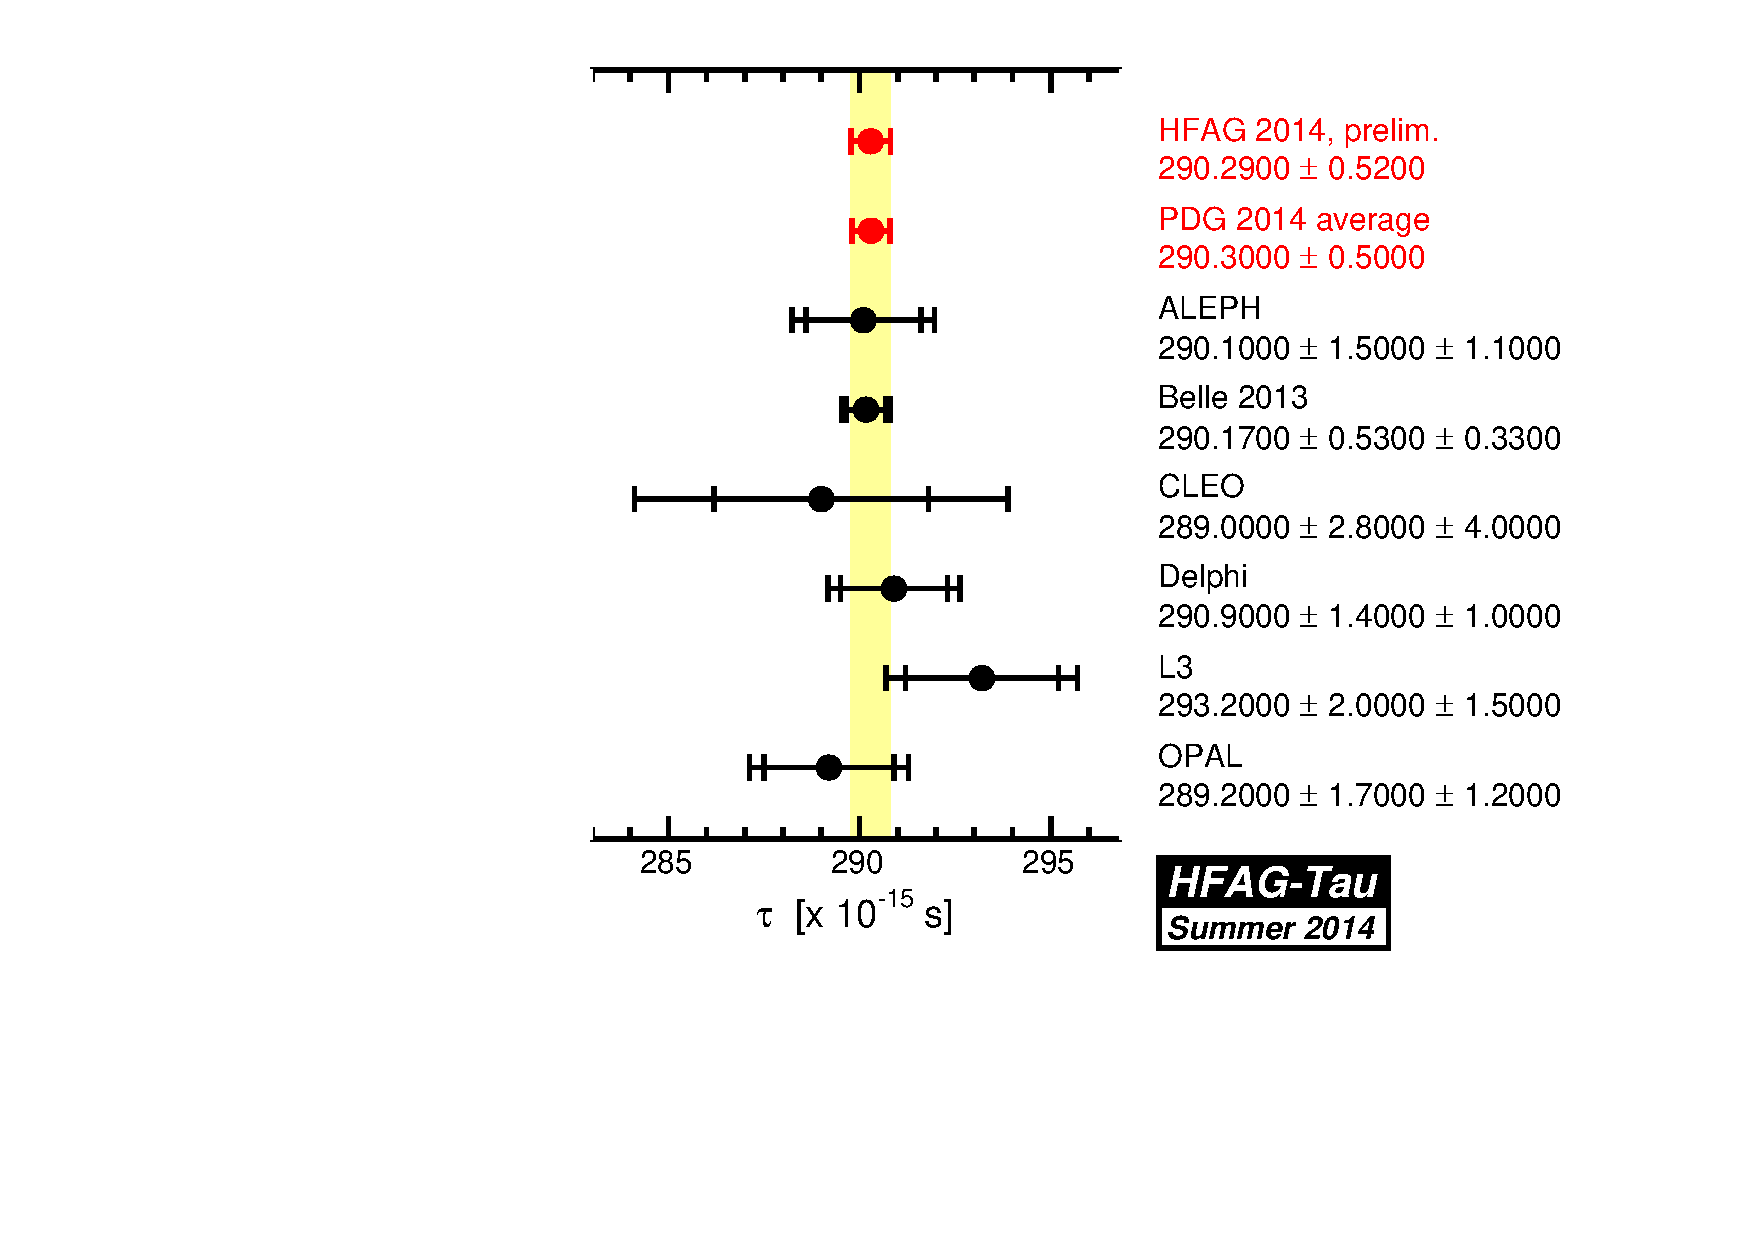
\includegraphics[width=0.66\linewidth,clip]{figures/tau/plot-taulife-hfag-summer2014}
    \fi
    \caption{\mtau lifetime average.%
      \label{fig:tau:tau-lifetime}%
    }
  \end{center}
\end{figure}

%% ///////////////////////////////////////////////////////////////////////////
\tausection{Tests of lepton universality}
\cutname{lepton-univ.html}
\label{sec:tau:leptonuniv}

Lepton universaility tests precision has significantly been improved by the
addition of the recent Belle \mtau lifetime
measurement~\cite{Belous:2013dba}, while improvements from the \mtau
branching fraction fit are negligible.
We compute the universality tests like in the previus report by using
proper ratios of the partial widths of a heavier lepton \lepth
decaying to a
lighter lepton \leptl~\cite{Marciano:1988vm},
\begin{align*}
  \Gamma(\lepth \to \nu_{\lepth} \leptl \nub_{\leptl} (\gamma)) =
  \frac{\BR(\lepth \to \nu_{\lepth} \leptl \nub_{\leptl})}{\tau_{\lepth}} =
  \frac {G_{\lepth} G_{\leptl} m^5_{\lepth}}{192 \pi^3}\, f\left(\frac {m^2_{\leptl}}{m^2_{\lepth}}\right)
  \opdelta^{\lepth}_W \opdelta^{\lepth}_\gamma~,
\end{align*}
where
\begin{alignat*}{3}
 G_{\leptl} &= \frac {g^2_{\leptl}}{4 \sqrt{2} M^2_W} &\quad&&
 f(x) &= 1 -8x +8x^3 -x^4 -12x^2 \text{ln}x \\
 \opdelta^{\lepth}_W &= 1 + \frac {3}{5} \frac {m^2_{\lepth}}{M^2_W} &\quad\quad&&
 \opdelta^{\lepth}_\gamma &= 1+\frac {\alpha(m_{\lepth})}{2\pi} \left(\frac {25}{4}-\pi^2\right)
\end{alignat*}
We use $\opdelta^\tau_\gamma=1-43.2\cdot 10^{-4}$ and
$\opdelta^\mu_\gamma=1-42.4\cdot 10^{-4}$~\cite{Marciano:1988vm} and $M_W$
from PDG 2013~\cite{PDG_2013} as usual.
We use HFAG 2014 averages and PDG 2013 for the other quantities.
Using pure leptonig processes we obtain
\begin{align*}
  \left( \frac{g_\tau}{g_\mu} \right) = \htuse{gtaubygmu_tau}~,
  && \left( \frac{g_\tau}{g_e} \right) = \htuse{gtaubyge_tau}~,
  && \left( \frac{g_\mu}{g_e} \right) = \htuse{gmubyge_tau}~.
\end{align*}
Using semi-hadronic processes
\begin{align*}
  \left( \frac{g_\tau}{g_\mu} \right)^2 =
  \frac{\BR({\tau \to h \nu_\tau})}{\BR({h \to \mu \bar{\nu}_\mu})}
  \frac{2m_h m^2_{\mu}\tau_h}{(1+\delta_{h})m^3_{\tau}\tau_{\tau}}
  \left( \frac{1-m^2_{\mu}/m^2_h}{1-m^2_h/m^2_{\tau}} \right)^2~,
\end{align*}
where $h$ = $\pi$ or $K$ and the radiative corrections are
$\delta_{\pi} = (\htuse{delta_LD_taupi_pimu}\%$ and
$\delta_{K} = (\htuse{delta_LD_tauK_Kmu}\%$~\cite{Decker:1994dd}.
we measure:
\begin{align*}
  \left( \frac{g_\tau}{g_\mu} \right)_\pi &= \htuse{gtaubygmu_pi}~,
  & \left( \frac{g_\tau}{g_\mu} \right)_K = \htuse{gtaubygmu_K}~.
\end{align*}
Similar tests could be performed with decays to electrons, however they are
less precise because the hadron two body decays to electrons are
helicity-suppressed.
Averaging the three \(g_\tau/g_\mu\) ratios we obtain
\begin{align*}
  \left( \frac{g_\tau}{g_\mu} \right)_{\tau{+}\pi{+}K} &= \htuse{gtaubygmu_fit}~,
\end{align*}
accounting for statistical correlations.
Table~\ref{tab:tau:univ-fit-corr} reports the statistical correlation coefficients for the fitted coupling ratios:
\ifhevea\begin{table}\fi%% otherwise cannot have normalsize caption
\begin{center}
\ifhevea
\caption{Universality coupling ratios correlation coefficients (\%)\label{tab:tau:univ-fit-corr}}%
\else
\begin{minipage}{\linewidth}
\begin{center}
\captionof{table}{Universality coupling ratios correlation coefficients (\%)}\label{tab:tau:univ-fit-corr}%
\fi
\begin{center}
\renewcommand*{\arraystretch}{1.1}%
\begin{tabular}{lcccc}
\toprule
\couplingsCorr
\\\bottomrule
\end{tabular}
\end{center}
\ifhevea\else
\end{center}
\end{minipage}
\fi
\end{center}
\ifhevea\end{table}\fi

%% ///////////////////////////////////////////////////////////////////////////
\tausection{Universality improved $\BR(\tau \to e \nu \bar{\nu})$ and $\Rhad$}
\cutname{Be_univ_and_Rtau.html}
\label{sec:tau:be_univ_rtau}

Following Ref.~\cite{Davier:2005xq}, we assume lepton universality to
obtain a more precise experimental determination of $\BR_e = \BR(\tau \to
e\bar{\nu}_e\nu_\tau)$ using the tau branching fraction to muon and the tau
lifetime. We average:
\begin{itemize}
\item the $\BR_e$ \htuse{Gamma5.td} fit value,
\item the $\BR_e$ determination from assuming that $g_\mu/g_e = 1$ hence (see
also Section~\ref{sec:tau:leptonuniv}) $\BR_e = \BR_\mu \cdot
f(m^2_e/m^2_\tau)/f(m^2_\mu/m^2_\tau)$,
\item  $\BR_e$ from assuming that $g_\tau/g_\mu =1$
hence $\BR_e = \BR(\mu \to e \bar{\nu}_e \nu_\mu)\cdot (\tau_\tau /
\tau_\mu) \cdot (m_\tau/m_\mu)^5 \cdot f(m^2_e/m^2_\tau)/f(m^2_e/m^2_\mu)
\cdot (\delta_\gamma^\tau \delta_W^\tau)/(\delta_\gamma^\mu \delta_W^\mu)$
where $\BR(\mu \to e \bar{\nu}_e \nu_\mu) = 1$.
\end{itemize}
Accounting for statistical correlations, we obtain
\begin{align*}
  \BR_e^{\text{uni}} = (\htuse{Be_univ})\%.
\end{align*}
The recent Belle \mtau lifetime measurement has brought a significant improvement.
We use $\BR_e^{\text{uni}}$ to obtain the ratio
\begin{align*}
  \Rhad = \frac{\Gamma(\tau \to \text{hadrons})}{\Gamma(\tau\to e\nu\bar{\nu})} = \htuse{R_tau}.
\end{align*}
Here $\Gamma(\tau \to \text{hadrons})$ is obtained by summing all tau
hadronic decay modes.

%% ///////////////////////////////////////////////////////////////////////////
\tausection{$\Vus$ measurement}
\cutname{vus.html}
\label{sec:tau:vus}

We have updated the CKM coefficient \Vus determinations of the previous
report using the updated data from HFAG 2014 and PDG 2013.

\tausubsection{Inclusive tau partial width to strange}

The tau hadronic partial width is the sum of the tau partial width to
strange and to non-strange hadronic final states,
$\Gammahad = \Gammastrange + \Gammanonstrange$.
Dividing by the partial width to electron, $\Gamma_e$, we obtain partial width ratios
(which are equal to the respective branching fraction ratios) for which
$\Rhad =  \Rstrange + \Rnonstrange$. In terms
of such ratios, \Vus is measured as
\begin{align*}
  \Vus &= \sqrt{\Rstrange/\left[\frac{\Rnonstrange}{\Vud^2} -  \delta R_{\text{theory}}\right]}~,
\end{align*}
where $\delta R_{\text{theory}}$ can be determined in the context of low
energy QCD theory, partly relying on experimental low energy scattering
data. We use $\delta R_{\text{theory}} =
\htuse{deltaR_su3break}$~\cite{Gamiz:2006xx}, which induces a systematic
error on \Vus that lies between two more recent estimates~\cite{Gamiz:2007qs,Maltman:2010hb}.

In the following, we use the universality improved $\BR_e^{\text{uni}}$
(see Section~\ref{sec:tau:be_univ_rtau}) to compute the $R$ ratios.
The most direct experimental determination of \Rstrange and $\Rnonstrange =
\Rhad-\Rstrange$ come from the tau inclusive branching fractions to
hadronic and strange hadronic states, $\BRhad$ and $\BRstrange$. However
often the total hadronic branching fraction has been replaced by the
indirect but more precise expression $\BRhad^{\text{uni}} = 1 - \BR_e
-\BR_\mu$ (or similar expressions based on $\BR_e^{\text{uni}}$), using
unitarity, see for example the 2009 HFAG report~\cite{Asner:2010qj}. We
depart from this choice here, and we use the most direct determination of
\Rhad, for two reasons: first there is no significant statistical gain in
the final errors, because of statistical correlations in the \Rhad
expression $(1-\BR_e -\BR_\mu)/\BR_e^{\text{univ}}$, and second the indirect
determination of $\Rnonstrange = \Rhad^{\text{uni}} - \Rstrange$ would
absorb the effect of possible unobserved hadronic states entirely in
\Rnonstrange, while they could also be strange final states.

With the above choices, using $\Vud = \htuse{Vud}$~\cite{Hardy:2008gy}, using
HFAG values of this report, including the above-mentioned
$\BR_e^{\text{univ}}$,
$\BRstrange = (\htuse{B_tau_s_fit})\%$ (see also Table~\ref{tab:tau:vus}),
$\BRnonstrange = (\htuse{B_tau_VA_fit})\%$
and the PDG 2013 averages, we obtain $\VusTauIncl = \htuse{Vus}$, which
is $\htuse{Vus_mism_sigma_abs}\sigma$ lower than the unitarity CKM
prediction $\VusUni = \htuse{Vus_uni}$, from $(\VusUni)^2 = 1 -
\Vud^2$. The \VusTauIncl uncertainty includes a systematic error
contribution of \htuse{Vus_err_th} from the theory uncertainty on
$\delta R_{\text{theory}}$,

If we use the alternative above mentioned
definitions of \BRhad, the mismatch is $+++3.4\sigma$.
Using a unitarity-constrained tau branching fraction fit, the mismatch is
$+++3.4\sigma$. The $\htuse{Vus_mism_sigma_abs}\sigma$ discrepancy is
+++close to the unconstrained fit result of the 2009 HFAG report,
$3.6\sigma$~\cite{Asner:2010qj}, and also to the $3.3\sigma$
from the \hfagtau 2011 intermediate document~\cite{Banerjee:2011az}, based
on a unitarity-constrained fit.

\iffalse
=== from \hfagtau 2011 report ===
Since the sum of base modes from our unconstrained fit is less than unity by $1.6~\sigma$,
instead of using $\B\Rnonstrange = 1 - \BR_{\text{leptonic}} - \B\Rstrange$,
we also evaluate $\Vus$ from the sum of the averaged non-strange branching fractions.
%Using our default method of not inflating the error bars on all the measurements,
This gives $\Vus$ $=$ $0.2169\, \pm\, 0.0023$, which is $3.5~\sigma$ lower than the CKM unitarity prediction.
\fi
%%
%% Gamma110 quantities
%%
\begin{table}
\begin{center}
\renewcommand*{\arraystretch}{1.3}%
\caption{HFAG Winter 2012 Tau branching fractions to strange final states.\label{tab:tau:vus}}%
\ifhevea\renewcommand{\bar}[1]{\textoverline{#1}}\fi
\begin{envsmall}
\begin{center}
\begin{tabular}{llll}
\hline
\multicolumn{1}{c}{\bfseries Branching fraction} &
\multicolumn{1}{c}{\bfseries HFAG Winter 2012 fit} \\
\hline
\HfagTauBrStrangeVal
\\\hline
\HfagTauBrStrangeTotVal
\\\hline
\end{tabular}
\end{center}
\end{envsmall}
\end{center}
\end{table}

\tausubsection{\Vus from $\BR(\tau \to K\nu) / \BR(\tau \to \pi\nu)$ and from $\BR(\tau \to K\nu)$}

We use the ratio of branching fractions $\BFtautoknu/\BFtautopinu = \htuse{Gamma10by5}$ to
measure \Vus from the equation
\begin{align*}
\frac{\BFtautoknu}{\BFtautopinu} &=
\frac{f_K^2 \Vus^2}{f_\pi^2 \Vud^2} \frac{\left( 1 - m_K^2/m_\tau^2 \right)^2}{\left( 1 -  m_\pi^2/m_\tau^2 \right)^2}
\frac{\opdelta_{\text{LD}}(\tau^- \to K^-\nut)}{\opdelta_{\text{LD}}(\tau^- \to \pi^-\nut)}~.
\end{align*}
In this ratio, the short-distance radiative corrections cancel.
The term $\opdelta_{\text{LD}}(p) = 1 + \delta_{\text{LD}}(p)$ corresponds to the
long-distance electroweak radiative correction factor for the process $p$.
Following Ref.~\cite{Banerjee:2008hg}, the ratio of radiative correction
factors is estimated as $\opdelta_{\text{LD}}^{K\pi} =
\opdelta_{\text{LD}}(\tau^- \to K^-\nu/K^- \to \mu^-\nu) /
\opdelta_{\text{LD}}(\tau^- \to \pi^-\nu/\pi^- \to \mu^-\nu) \cdot
\opdelta_{\text{LD}}(K^- \to \mu^-\nu)/\opdelta_{\text{LD}}(\pi^- \to \mu^-\nu)$,
where the first ratio is $[1+ (\htuse{delta_LD_tauK_Kmu})\%]/[1+
(\htuse{delta_LD_taupi_pimu})\%]$~\cite{Decker:1994ea} and the second ratio
is $(\htuse{rrad_LD_kmu_pimu})\%$~\cite{Marciano:2004uf}, hence assuming
independent errors $\opdelta_{\text{LD}}^{K\pi} =
\htuse{rrad_LD_tauK_taupi}$.
The ratio $f_K/f_\pi$ is estimated in lattice QCD to be \htuse{f_K_by_f_pi}~\cite{Aoki:2013ldr}.
We measure $\VusTauKpi = \htuse{Vus_tauKpi}$,
$\htuse{Vus_tauKpi_mism_sigma_abs}\sigma$ below the CKM unitarity prediction.

We use the branching fraction $\BFtautoknu$ to
measure \Vus from the equation
\begin{align*}
  \BR(\tau^- \to K^-\nu_\tau) =
  \frac{G^2_F f^2_K \Vus^2 m^3_{\tau} \tau_{\tau}}{16\pi\hbar} \left (1 - \frac{m_K^2}{m_\tau^2} \right )^2 S_{EW}~,
\end{align*}
where $f_K = \htuse{f_K}\,\mev$~\cite{Aoki:2013ldr} is the
kaon decay constant estimated with lattice QCD, and $S_{EW} = \htuse{rrad_tau_Knu}$~\cite{Erler:2002mv}
accounts for the radiative corrections. We obtain $\VusTauKnu =
\htuse{Vus_tauKnu}$, wich is $\htuse{Vus_tauKnu_mism_sigma_abs}\sigma$ below
the CKM unitarity prediction. CODATA 2010 results~\cite{Mohr:2012tt} and
PDG 2013 have been used for the physics constants.

\tausubsection{\Vus from tau summary}
\begin{figure}[tb]
  \begin{center}
   \ifhevea
    \begin{tabular}{@{}cc@{}}
      \larger\bfseries\ahref{hfag-tau-vus-plot.png}{PNG format} &
      \larger\bfseries\ahref{hfag-tau-vus-plot.pdf}{PDF format} \\
      \multicolumn{2}{c}{\ahref{hfag-tau-vus-plot.png}{%
          \imgsrc[alt="Vus summary plot"]{hfag-tau-vus-plot.png}}}
    \end{tabular}
    \else
    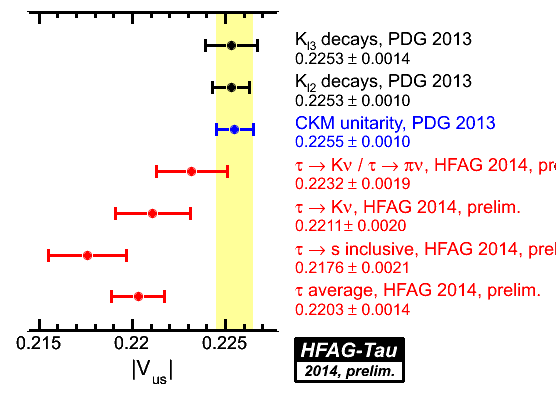
\includegraphics[width=0.66\linewidth,clip]{figures/tau/hfag-tau-vus-plot}
    \fi
    \caption{\Vus averages of this document compared with the FlaviaNet results~\cite{Antonelli:2010yf}.
      \label{fig:tau:vus-summary}%
    }
  \end{center}
\end{figure}

We summarize the \Vus results reporting the values, the discrepancy with
respect to the \Vus determination from CKM unitarity, and an illustration
of the measurement method:
\begin{alignat*}{6}
  &\VusUni &&= \htuse{Vus_uni} & \quad & & \quad
  & {\smaller\text{from } \sqrt{1 - \Vud^2} \quad\text{(CKM unitarity)}}~, \\
  %%
  &\VusTauIncl &&= \htuse{Vus} & \quad & \htuse{Vus_mism_sigma}\sigma &
  & {\smaller\text{from } \Gamma(\tau^- \to X_s^- \nut)}~, \\
  %%
  &\VusTauKpi &&= \htuse{Vus_tauKpi} & \quad & \htuse{Vus_tauKpi_mism_sigma}\sigma &
  & {\smaller\text{from } \Gamma(\tauknu)/\Gamma(\taupinu)}~,  \\
  %%
  &\VusTauKnu &&= \htuse{Vus_tauKnu} & \quad & \htuse{Vus_tauKnu_mism_sigma}\sigma &
  & {\smaller\text{from } \Gamma(\tauknu)}~.
\end{alignat*}

Thanks to the improved lattice QCD determination of
$f_K$~\cite{Aoki:2013ldr}, the uncertainty on
$\Vus_{\tau K}$ has been significantly reduced with respect to the
previous HFAG report. Averaging the three above \Vus determinations we
obtain:
\begin{alignat*}{6}
  & \Vus_\tau &&= \htuse{Vus_tau} &\quad &\htuse{Vus_tau_mism_sigma}\sigma \quad
  & \text{average of 3 \Vus tau measurements}.
\end{alignat*}
We could not find a published estimate of the correlation of the
uncertainties on $f_K$ and $f_K/f_\pi$, but even if we assume $\pm
100\%$ correlation, the uncertainty on $\Vus_\tau$ does not change
more than about $\pm 5\%$. Figure~\ref{fig:tau:vus-summary} summarizes the
\Vus results.
